% Le vélo d'hiver sur la rue de Terrebonne et les jours de chargement de la neige.
% Analyse des données du compteur communiquées en réponse à la demande d'accès
% 2026-300, jointes aux données météorologiques d'Environnement Canada et aux
% registres de déneigement de la Ville. Traduction de la version anglaise,
% qui fait foi. Compiler avec pdflatex (deux fois).
\documentclass[11pt,letterpaper]{article}
\usepackage[T1]{fontenc}
\usepackage[utf8]{inputenc}
\usepackage[scaled=0.95]{helvet}
\renewcommand{\familydefault}{\sfdefault}
\usepackage[letterpaper,top=0.9in,bottom=0.95in,left=1in,right=1in]{geometry}
\usepackage{microtype}
\usepackage{enumitem}
\usepackage{titlesec}
\usepackage{fancyhdr}
\usepackage{xcolor}
\usepackage{booktabs}
\usepackage{amsmath}
\usepackage{graphicx}
\usepackage{array}
\usepackage[hidelinks]{hyperref}
\urlstyle{same}
\newcommand{\docversion}{2026-10-16-16-30-24} % set by build (America/Toronto)
\hypersetup{pdfsubject={version \docversion}}

\setlength{\parindent}{0pt}
\setlength{\parskip}{0.5em}
\linespread{1.03}

\titleformat{\section}{\normalfont\large\bfseries}{\thesection}{0.6em}{}[\vspace{1pt}\titlerule]
\titlespacing*{\section}{0pt}{1.1em}{0.4em}
\titleformat{\subsection}{\normalfont\bfseries}{\thesubsection}{0.6em}{}
\titlespacing*{\subsection}{0pt}{0.8em}{0.25em}

\pagestyle{fancy}
\fancyhf{}
\renewcommand{\headrulewidth}{0pt}
\fancyfoot[C]{\footnotesize\color{gray}Demande d'accès 2026-300 -- vélo d'hiver et jours de chargement -- page \thepage}
\fancyfoot[R]{\tiny\color{gray}v.\,\docversion}

\newcommand{\repourl}{https://github.com/OpenMobilityData/Terrebonne-access-requests}
\newcommand{\repo}[1]{\href{\repourl}{#1}}
\newcommand{\doc}[2]{\href{\repourl/blob/main/#1}{#2}}
\newcommand{\pagesurl}{https://openmobilitydata.github.io/Terrebonne-access-requests}
\expandafter\def\csname bundle01\endcsname{2026-581/raw/01_emails_mandate_counts.pdf}
\newcommand{\pgl}[3]{\href{\pagesurl/\csname bundle#1\endcsname\#page=#2}{\textsf{\small[#1, p.~#3]}}}
\newcommand{\pg}[2]{\pgl{#1}{#2}{#2}}

\begin{document}

\begin{center}
{\Large\bfseries Le vélo d'hiver sur la rue de Terrebonne et les jours de chargement de la neige}\\[0.4em]
{\large Ce que montrent le compteur de l'arrondissement, Environnement Canada et les registres de déneigement de la Ville pour l'hiver 2025-2026}\\[0.6em]
Richard Hoge, Côte-des-Neiges--Notre-Dame-de-Grâce -- 13 octobre 2026\\
Traduction de la version anglaise, qui fait foi. Publié avec les données sources à \repo{\repourl}
\end{center}

\section*{Sommaire}

L'arrondissement de Côte-des-Neiges--Notre-Dame-de-Grâce a annoncé qu'une
direction de la piste cyclable protégée de la rue de Terrebonne sera
convertie en stationnement chaque hiver. Aucune date ne figure dans un
document de l'arrondissement\,; le conseiller de Loyola a décrit la saison
comme «\,December to March\,» et la réouverture comme fixée par «\,the data
and the weather\,» (CBC \emph{Daybreak}, 9~octobre 2026). La présente note
prend du 1\textsuperscript{er} décembre au 31 mars comme hiver. Le mandat
d'ingénierie à l'origine de l'annonce prévoyait
aussi une option plus étroite, la fermeture de la piste «\,en période de
déneigement seulement\,» \pg{01}{10}. La présente note mesure ce que
chacune de ces options aurait signifié pour les cyclistes l'hiver dernier,
à partir de trois sources publiques~: le compteur permanent de vélos de
l'arrondissement à l'angle de Terrebonne et de Kensington, communiqué en
réponse à la demande d'accès 2026-300\,; les données météorologiques
quotidiennes d'Environnement Canada\,; et le registre ouvert de la Ville de
Montréal de chaque chargement de camion de neige transporté hors de
l'arrondissement. Rien n'est modélisé\,; chaque chiffre est un comptage
d'une journée qui a eu lieu.

Deux constats ressortent. La plupart des journées d'hiver sont sans neige,
ce sont les journées où l'on roule le plus, et ces jours-là une voie de
stationnement à la place de la piste ne sert aucune fin liée à la neige,
tandis que chaque déplacement vers l'est se fait dans une voie de
circulation entre des voitures stationnées. Et les jours de neige, le vélo
se maintient près de son niveau hivernal habituel\,; ces jours-là la piste
serait fermée sous l'une ou l'autre option, et les déplacements se font
sur une chaussée au plus mauvais de son état.

\begin{enumerate}[nosep]
  \item \begin{minipage}[t]{\linewidth}\textbf{L'hiver dernier, 4~891 déplacements à vélo ont été comptés à
    Kensington entre le 1\textsuperscript{er} décembre et le 31 mars, dont
    2~783 vers l'est.} Sous une conversion de tout l'hiver, chaque
    déplacement vers l'est devient un déplacement en circulation mixte.
    Sous une fermeture limitée aux jours de chargement de la neige, le
    nombre est de 410 sur les jours de chargement de l'arrondissement
    (15~\%) et de 548 sur ceux du secteur de contrat qui contient
    Terrebonne (20~\%).\end{minipage}\vspace{0.35em}
  \item \begin{minipage}[t]{\linewidth}\textbf{La majeure partie du vélo d'hiver se fait les jours sans
    neige.} 1~699 déplacements vers l'est, soit 61~\%, ont eu lieu pendant
    les 67 journées sans aucune chute de neige\,; 83~\% pendant les
    journées de moins de 2,5~cm.\end{minipage}\vspace{0.35em}
  \item \begin{minipage}[t]{\linewidth}\textbf{Le résultat ne dépend pas de l'hiver.} L'hiver 2025-2026 a
    été léger~: 7,3~millions de m$^3$ de neige transportés dans toute la
    ville, le deuxième plus faible des onze saisons du registre municipal.
    L'application des calendriers de chargement de chacune de ces onze
    saisons aux comptages quotidiens de l'hiver dernier donne une part des
    jours de tempête de 9 à 24~\%, médiane 18~\%.\end{minipage}\vspace{0.35em}
  \item \begin{minipage}[t]{\linewidth}\textbf{Au c\oe ur de l'hiver, les jours de chargement voient autant
    de vélo que les autres.} De décembre à février, les déplacements vers
    l'est ont été en moyenne de 17 par jour les jours de chargement de
    l'arrondissement et de 18 les autres jours\,; l'écart sur toute la
    saison (17 contre 25) vient de mars, où l'usage augmente et la neige
    se fait rare. Les cyclistes d'hiver roulent pendant les opérations de
    chargement\,; ils ne restent pas chez eux pour elles.\end{minipage}\vspace{0.35em}
  \item \begin{minipage}[t]{\linewidth}\textbf{Le canal ouest du compteur s'est dégradé vers le
    1\textsuperscript{er} mars 2026.} Une caméra sur la même rue le
    confirme. Les chiffres ci-dessus traitent les comptages vers l'est
    comme des bornes inférieures à partir de cette date\,; sur la fenêtre
    sûre, du 1\textsuperscript{er} décembre au 28 février, les parts des
    jours de tempête sont de 23 et 28~\% et la part des jours sans neige
    de 48~\%. Les conclusions sont les mêmes sur l'une ou l'autre
    fenêtre.\end{minipage}
\end{enumerate}

\section{Données}

\textbf{Comptages de vélos.} L'arrondissement exploite un compteur à
boucle inductive Eco-Compteur ZELT EVO sur Terrebonne à Kensington, en
service depuis le 26~juillet 2025. Son relevé horaire par direction, du
26~juillet 2025 au 11~mai 2026, a été communiqué le 4~juin 2026 en réponse
à la demande d'accès 2026-300 (\doc{2026-300/raw/}{raw/})\,; la
documentation de l'équipement a été communiquée en réponse à la demande
2025-697. Additionné par jour, le relevé correspond exactement aux totaux
quotidiens que l'arrondissement a communiqués le 9~octobre 2026 dans le
dossier 2026-581 \pgl{01}{74}{74--81}~: du 1\textsuperscript{er} décembre
au 31 mars, 4~891 déplacements, 2~783 vers l'est et 2~108 vers l'ouest. Sur
la première année complète du compteur, du 26~juillet 2025 au 25~juillet
2026, le même tableau quotidien donne 135~276 passages de vélos (371 par
jour) et 501~817 véhicules motorisés (1~375 par jour)~: un vélo pour
3,7~véhicules motorisés, soit 21\,\% de tous les véhicules comptés. Le
chiffre des vélos est une borne inférieure~: les 29, 30 et 31~mai 2026
sont trois journées à zéro (une panne), et la détection du canal vers
l'ouest s'est dégradée vers le 1\textsuperscript{er}~mars 2026 (voir
Limites). La
direction est est prise ici comme celle qui perdrait sa piste~: à
l'émission \emph{Daybreak} de CBC, le 9~octobre, le conseiller de Loyola a
dit que l'orientation donnée aux services était «\,to favour the side that
will be against traffic to remain during winter\,» [00:38], comme il l'avait
dit en réponse à des questions à la séance du 6~octobre et auparavant à
l'APC-NDG\,; la piste allant dans le même sens que la circulation
automobile est, à Kensington, la direction est (à l'ouest de Cavendish, où
le sens unique s'inverse, c'est la direction ouest). Si c'était la piste vers l'ouest qui était
convertie, chaque chiffre se multiplierait par 2~108/2~783 et aucune
conclusion ne changerait.

\textbf{Météo.} Données quotidiennes d'Environnement et Changement
climatique Canada pour l'aéroport international Pierre-Elliott-Trudeau de
Montréal (identifiant climatologique 7025251)~: chute de neige totale,
neige au sol, température.\footnote{Données climatiques historiques
d'ECCC, \url{https://climate.weather.gc.ca}\,; les deux fichiers annuels
sont dans \doc{2026-300/derived/}{derived/}.} Une journée manquante
(8~mars) est traitée comme sans neige.

\textbf{Chargement de la neige.} La Ville publie chaque chargement de
camion de neige avec son heure de chargement, son secteur de contrat, son
arrondissement, son site de dépôt et son volume (\emph{Contrats et
transactions de déneigement}, CC-BY
4.0).\footnote{\url{https://donnees.montreal.ca/dataset/contrats-transaction-deneigement}}
Filtré sur le code d'arrondissement CDN et additionné par jour, il donne
les jours de chargement de l'arrondissement pour chaque saison depuis
2015-2016. Les polygones de secteurs de la Ville pour
2025-2026\footnote{\emph{Secteurs de déneigement},
\url{https://donnees.montreal.ca/dataset/secteur-deneigement}.} placent la
piste dans le secteur de contrat CDN-301 depuis son extrémité ouest, juste
à l'ouest de Belmore, jusqu'entre Royal et Draper, soit environ 1,8 de ses
2,4~km, compteur compris\,; les derniers tronçons, de Draper à Girouard
(environ 0,55~km), sont dans le secteur CDN-111, et l'intersection
Girouard se trouve sur la limite avec CDN-112 (intersections tirées de la
géobase de la Ville\,; la vérification est \texttt{terrebonne\_sector.py}).
Une journée de 100 chargements ou plus dans l'arrondissement, ou
de 40 ou plus dans le secteur, est comptée comme jour de chargement\,; les
opérations complètes atteignent plusieurs centaines de chargements par
jour et les queues sous ces seuils sont des reprises. En 2025-2026, cela
donne 24 jours de chargement de l'arrondissement en six épisodes (12 au
16 et 28 au 31~décembre, 8 et 9, 17 au 21 et 27 au 31~janvier, 27~février
au 2~mars), qui correspondent aux six opérations annoncées par la Ville,
et 30 jours pour le secteur CDN-301, dont les opérations durent un ou deux
jours de plus.

\section{Méthode}

Soit $n_d$ le nombre de déplacements vers l'est comptés le jour $d$ de la
saison $S$ (du 1\textsuperscript{er} décembre au 31 mars, 121 jours). Sous
une conversion de tout l'hiver, l'exposition est $E_{\text{tout}} =
\sum_{d\in S} n_d = 2~783$. Sous une fermeture limitée à un ensemble de
jours de tempête $\mathcal{D}$, elle est $E_{\mathcal{D}} =
\sum_{d\in\mathcal{D}} n_d$. Comme la Ville n'a pas dit comment une
fermeture de tempête serait définie, $\mathcal{D}$ est calculé selon
plusieurs définitions, d'une seule journée de neige à chaque journée
comportant une activité de chargement dans l'arrondissement. Pour vérifier
la dépendance à l'hiver, les calendriers de chargement CDN de chacune des
onze saisons sont aussi appliqués, par date du calendrier, aux comptages
de 2025-2026~: les mêmes cyclistes, un autre calendrier de tempêtes.

\section{Résultats}

\begin{table}[htbp]
\centering\footnotesize
\begin{tabular}{p{8.6cm}rrr}
\toprule
Règle de fermeture & Jours & Dépl.\ vers l'est & Part \\
\midrule
\textbf{Tout l'hiver, 1\textsuperscript{er}~décembre -- 31~mars} & \textbf{121} & \textbf{2~783} & \textbf{100~\%} \\[2pt]
Jours de chargement de l'arrondissement ($\geq$100 chargements) & 24 & 410 & 15~\% \\
Jours de chargement du secteur CDN-301 ($\geq$40) & 30 & 548 & 20~\% \\
De la chute déclenchante ($\geq$2,5~cm) à la fin du chargement (arrondissement) & 36 & 592 & 21~\% \\
De la chute déclenchante à la fin du chargement (secteur CDN-301) & 44 & 770 & 28~\% \\
Toute journée avec activité de chargement dans l'arrondissement & 59 & 1~129 & 41~\% \\
Toute journée avec activité de chargement dans le secteur CDN-301 & 36 & 600 & 22~\% \\
Toute journée de $\geq$2,5~cm de neige & 24 & 462 & 17~\% \\
Journée de $\geq$2,5~cm et le lendemain & 44 & 843 & 30~\% \\
Journée de $\geq$5~cm et les quatre jours suivants & 66 & 1~219 & 44~\% \\
Toute journée de neige mesurable & 54 & 1~084 & 39~\% \\
\midrule
\multicolumn{4}{l}{\emph{Fenêtre sûre, 1\textsuperscript{er}~décembre -- 28~février (90 jours\,; 1~626 dépl.\ vers l'est)}} \\
Jours de chargement de l'arrondissement ($\geq$100 chargements) & 22 & 380 & 23~\% \\
Jours de chargement du secteur CDN-301 ($\geq$40) & 26 & 450 & 28~\% \\
De la chute déclenchante à la fin du chargement (secteur CDN-301) & 40 & 672 & 41~\% \\
Toute journée de $\geq$2,5~cm de neige & 19 & 322 & 20~\% \\
\bottomrule
\end{tabular}
\caption{Déplacements à vélo vers l'est à Terrebonne/Kensington qui
auraient été faits en circulation mixte selon chaque règle de fermeture,
hiver 2025-2026. Compteur~: demande 2026-300. Neige~: ECCC,
Montréal--Trudeau. Chargement~: jeu de données des transactions de la
Ville, arrondissement CDN et secteur CDN-301.}\label{tab:season}
\end{table}

\begin{figure}[htbp]
\centering
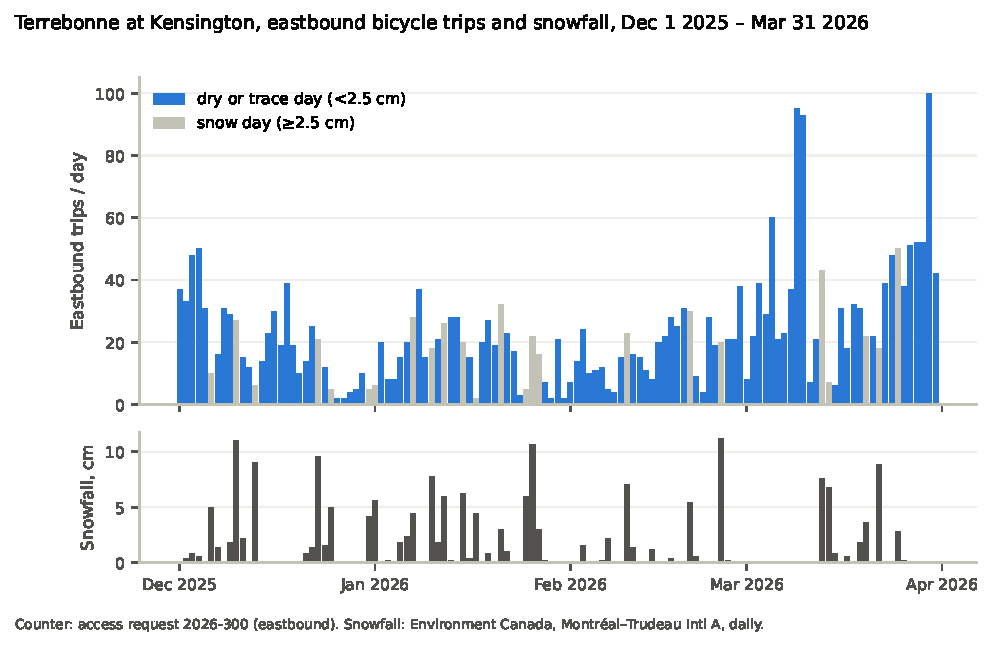
\includegraphics[width=\linewidth]{exposure_winter_2025-26.pdf}
\caption{Déplacements quotidiens vers l'est (haut) et chute de neige
(bas), du 1\textsuperscript{er} décembre 2025 au 31 mars 2026. Les barres
grises marquent les journées de 2,5~cm de neige ou plus. (Légende en
anglais~: \emph{dry or trace day}, journée sèche ou de traces\,;
\emph{snow day}, journée de neige.)}
\end{figure}

\begin{table}[htbp]
\centering\footnotesize
\begin{tabular}{p{7.6cm}rrr}
\toprule
Saison dont le calendrier de chargement CDN est appliqué & Jours de chargement & Dépl.\ vers l'est & Part \\
\midrule
2015-2016 & 21 & 481 & 17~\% \\
2016-2017 & 30 & 550 & 20~\% \\
2017-2018 (la plus lourde du registre, 18,0~M~m$^3$) & 42 & 639 & 23~\% \\
2018-2019 & 40 & 673 & 24~\% \\
2019-2020 & 24 & 443 & 16~\% \\
2020-2021 & 21 & 399 & 14~\% \\
2021-2022 & 27 & 527 & 19~\% \\
2022-2023 & 27 & 517 & 19~\% \\
2023-2024 (la plus légère, 6,5~M~m$^3$) & 12 & 247 & 9~\% \\
2024-2025 & 27 & 503 & 18~\% \\
2025-2026 (7,3~M~m$^3$) & 24 & 410 & 15~\% \\
\bottomrule
\end{tabular}
\caption{Les comptages quotidiens de 2025-2026 sous le calendrier de
chargement de l'arrondissement de chaque saison ($\geq$100 chargements par
jour, alignés par date du calendrier). Seul le calendrier des tempêtes
change d'une ligne à l'autre.}
\end{table}

\textbf{Les jours de tempête sont une minorité des déplacements.} Sur les
jours de chargement mesurés de l'arrondissement, une fermeture limitée aux
tempêtes aurait placé 410 déplacements vers l'est en circulation mixte,
soit 15~\% des 2~783 que touche une conversion de tout l'hiver\,; sur ceux
du secteur, 548 (20~\%)\,; en remontant jusqu'à la chute de neige
déclenchante, 592 (21~\%)\,; sur chaque journée comportant la moindre
activité de chargement, 1~129 (41~\%). Sous la règle la plus généreuse du
tableau, 44~\%. Toutes les définitions laissent plus de la moitié de
l'exposition de tout l'hiver sous forme de déplacements faits des jours
où aucune fermeture de tempête ne se serait appliquée.

\textbf{La majeure partie du vélo d'hiver se fait les jours secs.} Des
2~783 déplacements vers l'est, 1~699 (61~\%) ont eu lieu pendant les 67
journées sans aucune chute de neige, et 2~321 (83~\%) pendant les 97
journées de moins de 2,5~cm. Sur la fenêtre de décembre à février, 775 sur
1~626 (48~\%) ont eu lieu les jours sans neige.

\textbf{Les cyclistes roulent les jours de neige et pendant les opérations
de chargement.} Sur la saison, la moyenne des déplacements vers l'est a
été de 25,4 les jours secs, de 20,7 les jours de traces et de 19,2 les
jours de 2,5~cm ou plus, et de 17,1 les jours de chargement de
l'arrondissement contre 24,5 les autres jours. L'essentiel de cet écart
est mars~: sur la fenêtre de décembre à février, les chiffres sont de 17,2
les jours secs, 16,9 les jours de $\geq$2,5~cm, et 17,3 les jours de
chargement contre 18,3 les autres jours. D'un jour à l'autre, les
déplacements sont davantage corrélés à la température moyenne ($+0{,}54$
sur la saison) et à la neige au sol ($-0{,}44$) qu'à la chute du jour
($-0{,}12$)~: le froid et la neige accumulée freinent le vélo plus que la
chute du jour. Les exceptions sont les tempêtes les plus fortes~:
l'opération du 27 au 31~janvier, qui a suivi 16,6~cm en trois jours, a vu
2, 7 et 2 déplacements trois de ses cinq jours.

\textbf{L'hiver ne change pas la réponse.} L'hiver 2025-2026 a été léger,
185~cm à Trudeau contre une moyenne de longue durée voisine de 210, sans
journée au-delà de 11,2~cm et avec 7,3~millions de m$^3$ transportés dans
toute la ville, le deuxième plus faible des onze saisons (médiane 12,0\,;
2017-2018, 18,0). Le second tableau applique les calendriers de chargement
des dix autres saisons aux mêmes comptages quotidiens~: la part va de 9 à
24~\%, médiane 18~\%, et la saison la plus lourde du registre donne 23~\%.
À l'échelle du secteur, les onze saisons donnent de 8 à 23~\%.

\section{En bref}

\textbf{Les jours secs, la conversion coûte aux cyclistes et ne soulage
aucune contrainte liée à la neige.} Soixante et un pour cent des
déplacements vers l'est de l'hiver dernier (1~699\,; 48~\% sur la fenêtre
de décembre à février) ont été faits des jours sans chute de neige, où
l'offre de stationnement de la rue n'est pas réduite par les bancs de
neige et où aucune opération de chargement n'est en cours. Sous une
conversion de tout l'hiver, chacun de ces déplacements se fait dans
l'unique voie de circulation restante, entre des voitures stationnées des
deux côtés, avec les dangers propres à cette configuration~: moins
d'espace pour dépasser, et l'ouverture des portières tout le long du
tronçon. Sous une fermeture limitée aux tempêtes, aucun n'est touché. Ce
que la conversion procure ces jours-là, c'est du stationnement un jour où
le stationnement ne manque pas d'espace à cause de la neige\,; savoir si
cela vaut l'exposition est un jugement que cette note ne porte pas, mais
les quantités de part et d'autre sont maintenant connues.

\textbf{Les jours de neige, le vélo continue, et l'exposition par
déplacement est plus grande.} Au c\oe ur de l'hiver, les jours de chargement
ont porté autant de déplacements vers l'est que les autres jours (17
contre 18 par jour, de décembre à février). Ce sont les jours de traction
et de visibilité réduites, où la marge entre un vélo et un véhicule qui le
dépasse compte le plus. Sous l'une ou l'autre option, la piste est
indisponible ces jours-là\,; la différence entre les options tient tout
entière dans les jours secs ci-dessus. Une fermeture confinée aux jours de
chargement placerait donc les déplacements en circulation mixte exactement
les jours où la chaussée est au pire, et nulle part ailleurs\,; la
conversion de tout l'hiver y ajoute le reste de la saison.

\textbf{Sous forme d'hypothèse.} Si la proposition actuelle avait été en
vigueur l'hiver dernier, et en supposant que la nouvelle configuration
n'aurait pas dissuadé les cyclistes de circuler sur Terrebonne, comme on
l'a prédit à la séance du conseil du 6~octobre, on peut poser les effets
suivants~:
\begin{enumerate}[nosep]
  \item les 67 jours sans neige, 1~699 déplacements à vélo auraient été
    déplacés d'une piste cyclable protégée vers une voie de circulation,
    peut-être plus étroite qu'aujourd'hui, bordée de voitures stationnées
    des deux côtés\,;
  \item les 54 autres jours, 1~084 déplacements à vélo faits des jours de
    chute de neige auraient été déplacés vers la voie de circulation
    partagée.
\end{enumerate}
La mesure est confinée à l'hiver, et pourtant plus de la moitié des jours
de l'hiver dernier, 67 sur 121, n'ont eu aucune chute de neige. Un jour
sec peut suivre une tempête alors que les bancs de neige ne sont pas
encore enlevés\,; en comptant comme jour où la neige contraint le
stationnement chaque jour depuis une chute déclenchante de 2,5~cm ou plus
jusqu'à la fin de l'opération de chargement qui a suivi dans le secteur de
déneigement de Terrebonne, CDN-301, on obtient 44 de ces jours et 770
déplacements, et il reste 77 jours (64~\%) et 2~013 déplacements (72~\%)
où la piste aurait été du stationnement sans neige dans la rue pour le
justifier. La même règle appliquée aux jours de chargement de
l'arrondissement, qui se terminent un jour ou deux plus tôt, donne 36 jours
à l'intérieur et 85 jours (70~\%) et 2~191 déplacements (79~\%) à
l'extérieur (tableau~\ref{tab:season}).
Les hypothèses sont celles de la note~: les déplacements sont les passages
vers l'est à Kensington, la direction que le conseiller a dit devoir être
convertie, et un plancher de l'usage de la rue\,; la chute de neige est le
total du jour à l'aéroport Trudeau, et les jours sans neige comprennent des
jours avec de la neige au sol\,; la largeur de la voie de circulation dans
l'aménagement hivernal ne figure pas dans les documents communiqués.

\section{Limites}

\textbf{Le compteur à partir du 1\textsuperscript{er} mars 2026.} Les
totaux vers l'est et vers l'ouest du compteur s'équilibrent à quelques
pour cent près chaque mois de juillet 2025 à février 2026 et divergent à
partir de mars (70~\% vers l'est en mars, 59 à 61~\% en avril et en mai).
La caméra citoyenne Telraam de Terrebonne à King-Edward, qui observe la
même chaussée, concorde avec le canal est de la boucle jusqu'en mars mais
enregistre des journées de 80 à 190 vélos vers l'ouest là où la boucle en
enregistre 10 à 40, après quatre mois où la boucle comptait 1,6 à 2 vélos
vers l'ouest pour chacun que voyait la caméra. La détection vers l'ouest
de la boucle s'est donc dégradée vers le 1\textsuperscript{er} mars, et
ses comptages à partir de cette date sont des bornes inférieures. Les
chiffres de mars vers l'est concordent avec la caméra mais ne sont pas
garantis séparément, raison pour laquelle le tableau donne aussi la
fenêtre de décembre à février. Interrogée le 13~octobre 2026 sur un
éventuel entretien, déplacement ou réglage du compteur, la division de
l'ingénierie de l'arrondissement a répondu le 15~octobre qu'aucune
intervention n'a eu lieu sur la boucle entre la mi-février et la mi-mars
2026, que la seule intervention répertoriée est un remplacement de pile au
début de juin, avec une brève interruption dont les données ont été
reconstituées par le fabricant, qu'elle ne voit aucun indice de
défaillance technique, et qu'un amas de neige ou de glace du côté ouest,
le côté des voitures stationnées, a pu modifier la trajectoire des
cyclistes. Le relevé hebdomadaire situe la rupture dans la semaine du
2~mars et montre que le déséquilibre persiste à 58--61~\% vers l'est en
avril et au début de mai, une fois la neige disparue, alors que la
répartition directionnelle de la caméra bouge peu sur les mêmes mois\,;
les comptages vers l'ouest à partir du 1\textsuperscript{er}~mars restent
donc ici des bornes inférieures.

\textbf{Un hiver, une station, un compteur.} Le compteur se trouve en un
point d'une piste de 2,45~km\,; l'usage varie le long de celle-ci.
L'aéroport Trudeau est à 12~km à l'ouest de Terrebonne\,; les chutes de
neige d'une journée sont bien corrélées d'un bout à l'autre de l'île, mais
les quantités sur les rues de NDG peuvent différer. Les jours de
chargement sont ceux de l'arrondissement et du secteur CDN-301\,; les
derniers tronçons de la piste, de Draper à Girouard, sont dans le secteur
CDN-111 et hors des chiffres du secteur, et les limites des secteurs
peuvent avoir changé d'un contrat à
l'autre (seuls les polygones de 2025-2026 ont été vérifiés\,; CDN-301
apparaît sous les noms 301A et 301B en 2019-2020 et est combiné). Le
tableau multi-saisons maintient les cyclistes fixes et ne change que le
calendrier\,; dans un hiver plus lourd, moins de gens auraient roulé les
jours de tempête eux-mêmes, ce qui rend ces lignes prudentes dans l'autre
sens.

\textbf{Ce que cette note ne mesure pas.} Le côté stationnement~: combien
de cases sont perdues aux bancs de neige quels jours, et combien de
véhicules en ont besoin. Le registre de la Ville ne contient aucun
comptage de ce genre. Cette note mesure ce qu'aurait été le côté cycliste
d'une fermeture de tout l'hiver et d'une fermeture limitée aux
tempêtes\,; la comparaison des avantages appartient au lecteur.

\section{Fichiers}

Tous les intrants et le script qui produit chaque chiffre ci-dessus sont
dans \doc{2026-300/derived/}{2026-300/derived/}~: le relevé du compteur
additionné par jour et par direction\,; le tableau quotidien fusionné avec
la météo et l'activité de chargement\,; le registre de chargement de la
Ville additionné par saison, jour, arrondissement et secteur\,; les deux
fichiers annuels d'ECCC\,; la recherche de secteur\,; et
\texttt{exposure\_analysis.py}, qui régénère les tableaux et la figure à
partir de ces fichiers. Le classeur horaire du compteur et la lettre de
réponse de l'arrondissement sont dans \doc{2026-300/raw/}{2026-300/raw/},
tels que reçus.

\end{document}
